\documentclass[12pt,a4paper]{article}
\usepackage{geometry}
\geometry{left=2.54cm, right=2.54cm, top=2.98cm, bottom=2.98cm}
\usepackage{fancyhdr} 
\usepackage{enumerate}
\usepackage{graphicx}
\usepackage{subfigure}
\usepackage{caption}
\usepackage{float}
\usepackage{indentfirst}
\usepackage{threeparttable}
\usepackage{longtable}
\usepackage{hyperref}
\usepackage{setspace}
\hypersetup{
	colorlinks=true,
	linkcolor=black,
	filecolor=black,      
	urlcolor=black,
	citecolor=black,
}
\title{Projectile Motion}
\author{ZHANGYIHENG 10.7 27}
\date{}
\begin{document}
\begin{spacing}{1.25}
\maketitle
\tableofcontents
\setlength{\parindent}{4ex}
\newpage

\section{Intro}
\subsection{Definition of Projectile Motion}
Projectile motion is the motion of an object thrown (projected) into the air when, after the initial force that launches the object, air resistance is negligible and the only other force that object experiences is the force of gravity.
\subsection{Objective}
The purpose of the experiment is to gain a better and deeper understanding of the projectile motion in life. With the help of video analysis provided by Logger Pro, we can easily determine different physical quantities of the 2-D projectile motion, such as its \(V_a\), \(V_h\), \(h_{max}\), etc. In this case, we would simplify the motion into vertical as well as horizontal ones.
\subsection{Apparatuses}
\begin{enumerate}
    \setlength{\itemsep}{1ex}
    \item Digital camera
    \item Blackboard with lattices 
    \item Metal ball
    \item Logger Pro.
    \setlength{\topsep}{1ex}
\end{enumerate}
\newpage
\section{Procedure}
\subsection{Data Collecting}
Our aim was to investigate the motion of the ball and determine its trajectory. During our physics experiment, my partner and I took turns throwing a metal ball in front of a blackboard while the other recorded its projectile motion.\par
After recording the video, we loaded it into Logger Pro, which allowed us to obtain the trajectory of the ball during motion. We then turned the locus into a series of coordinates, which we recorded in a data table. The data table is included in the appendixes.\par
\subsection{Analysis}
\subsubsection{Horizontal Component}
\begin{figure}[H]
    \centering
    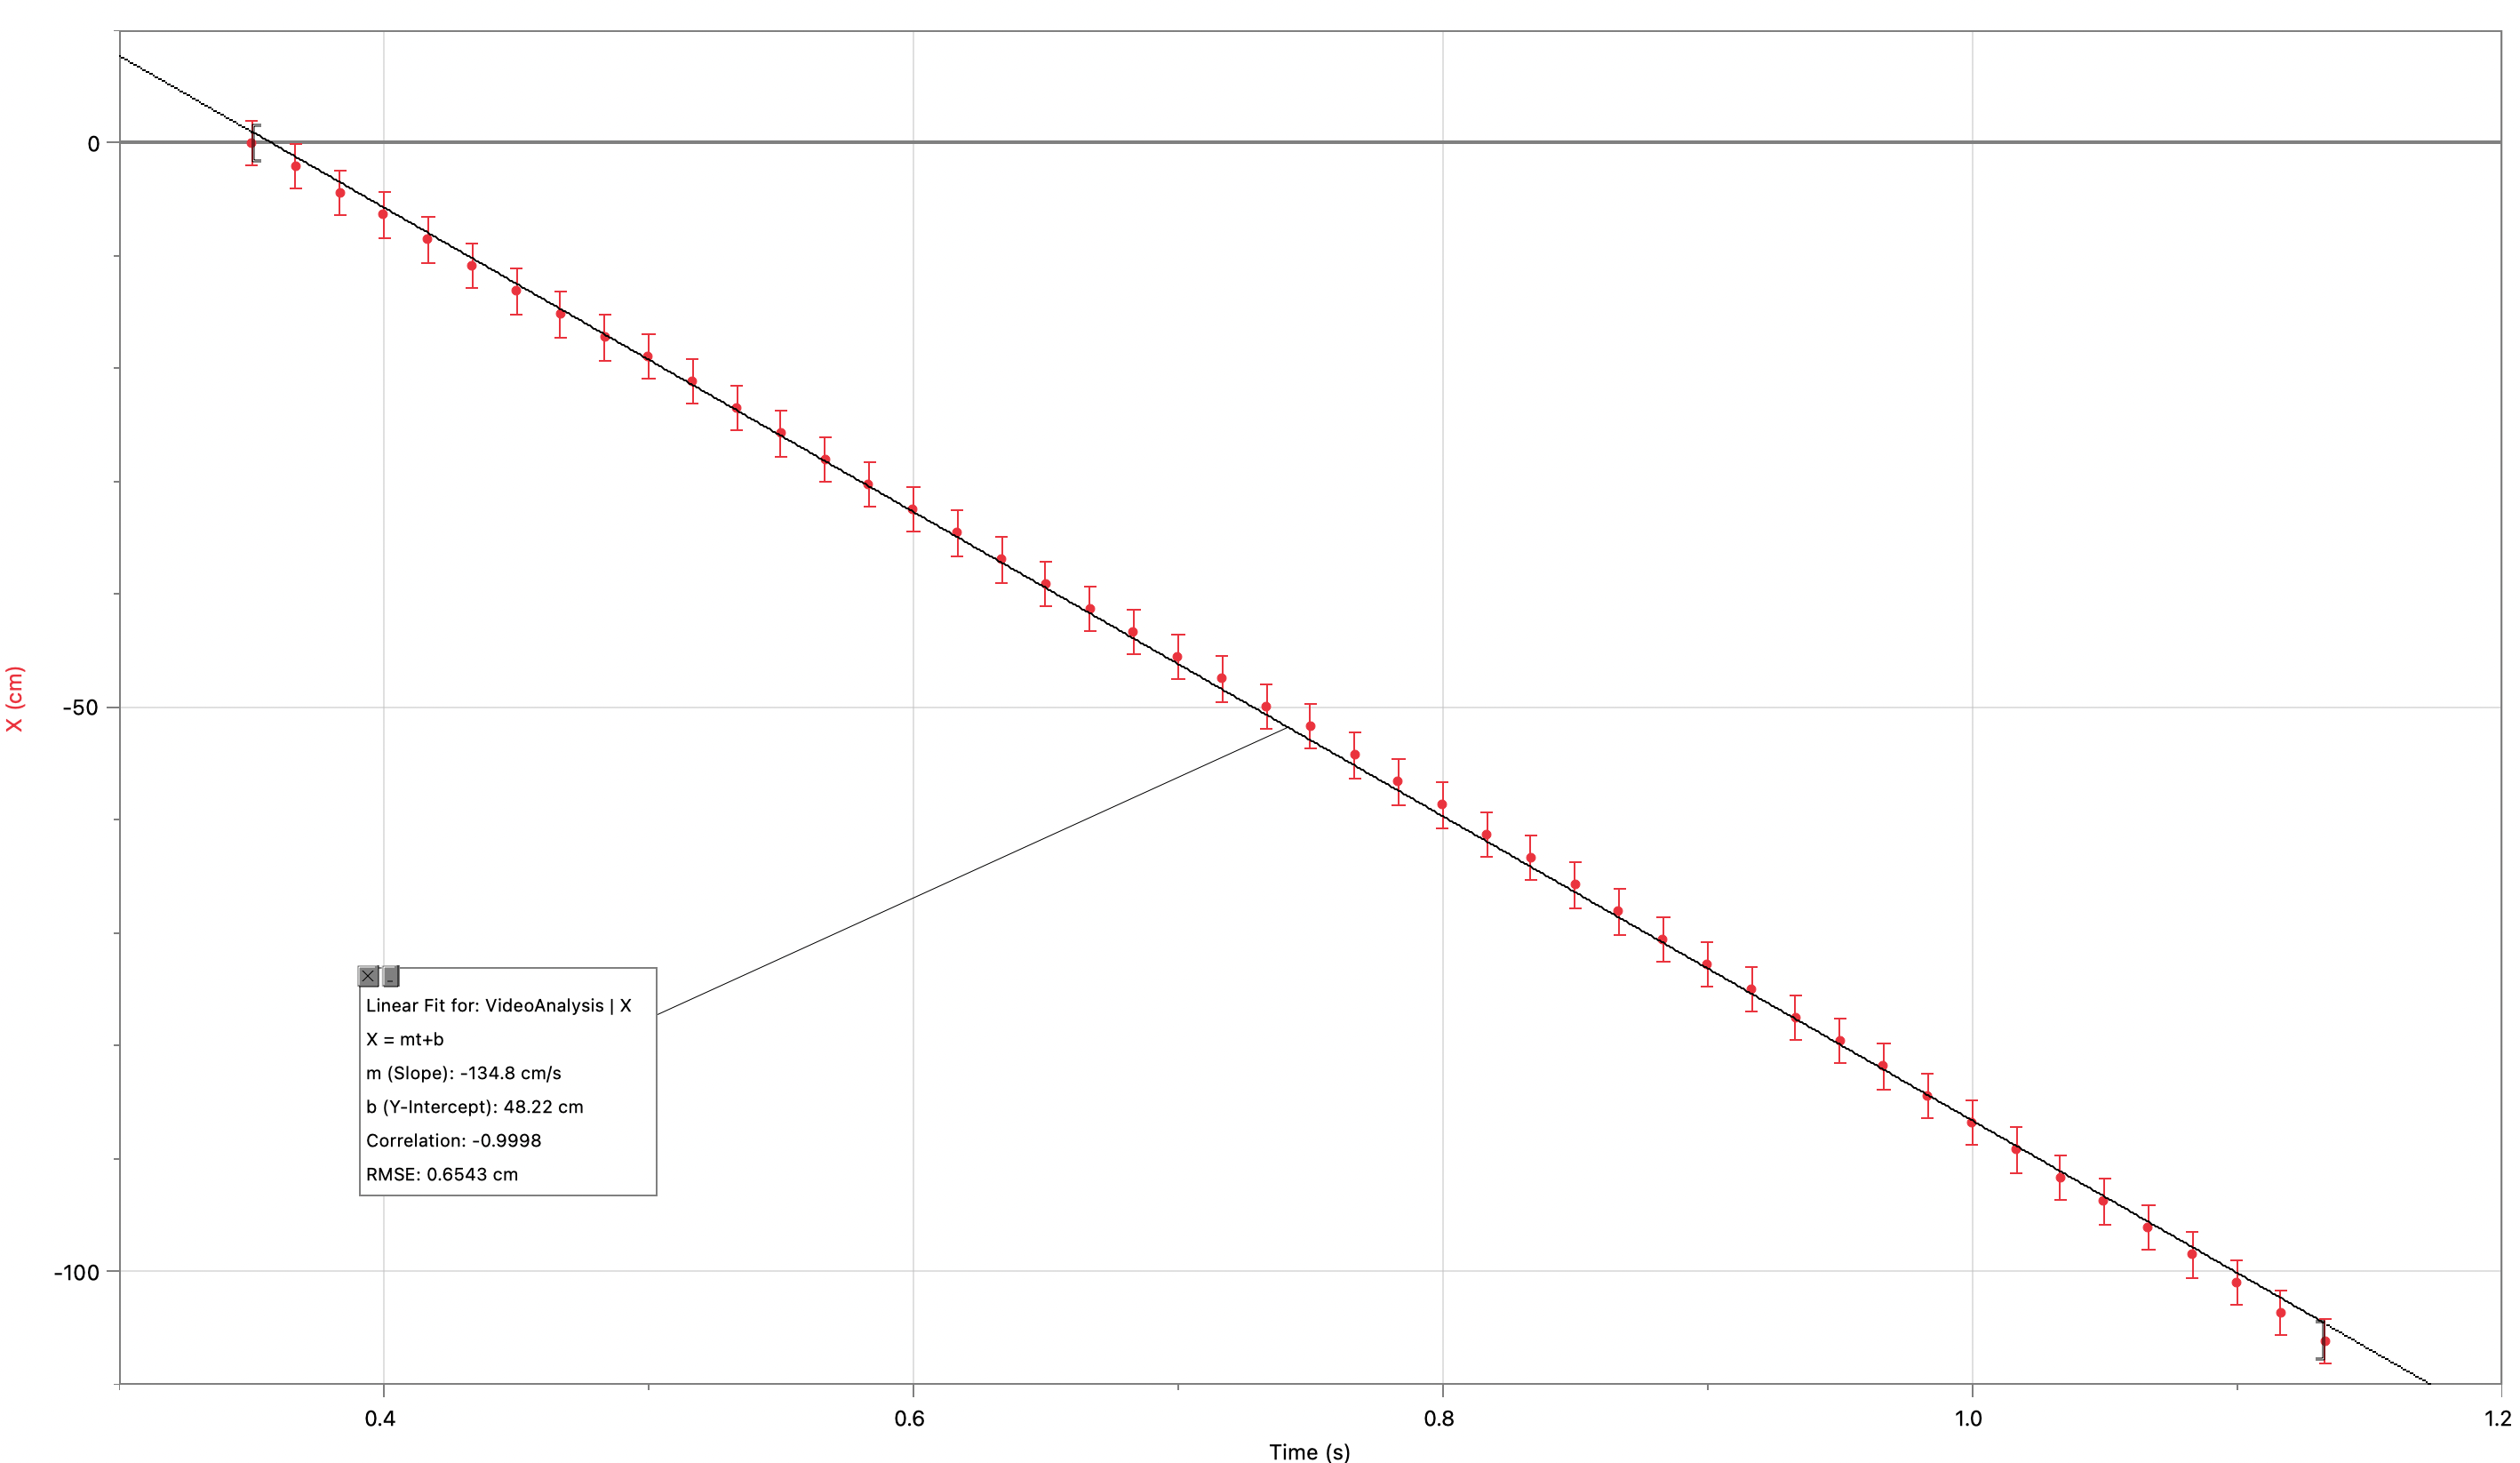
\includegraphics[width=15.9cm, height=10.8cm]{Sx-t.png}
    \caption{\(S_x\)-$t$ Graph}
    \label{fig1}
\end{figure}
Using data collected in Logger Pro, we could draw a \(S_x\)-t graph as shown.\par
Clearly, \(S_x\) and time satisfy a linear relationship. According to Logger Pro, their relationship is
\[
    S_x = -134.8t + 48.22
\]
\subsubsection{Vertical Component}
\begin{figure}[H]
    \centering
    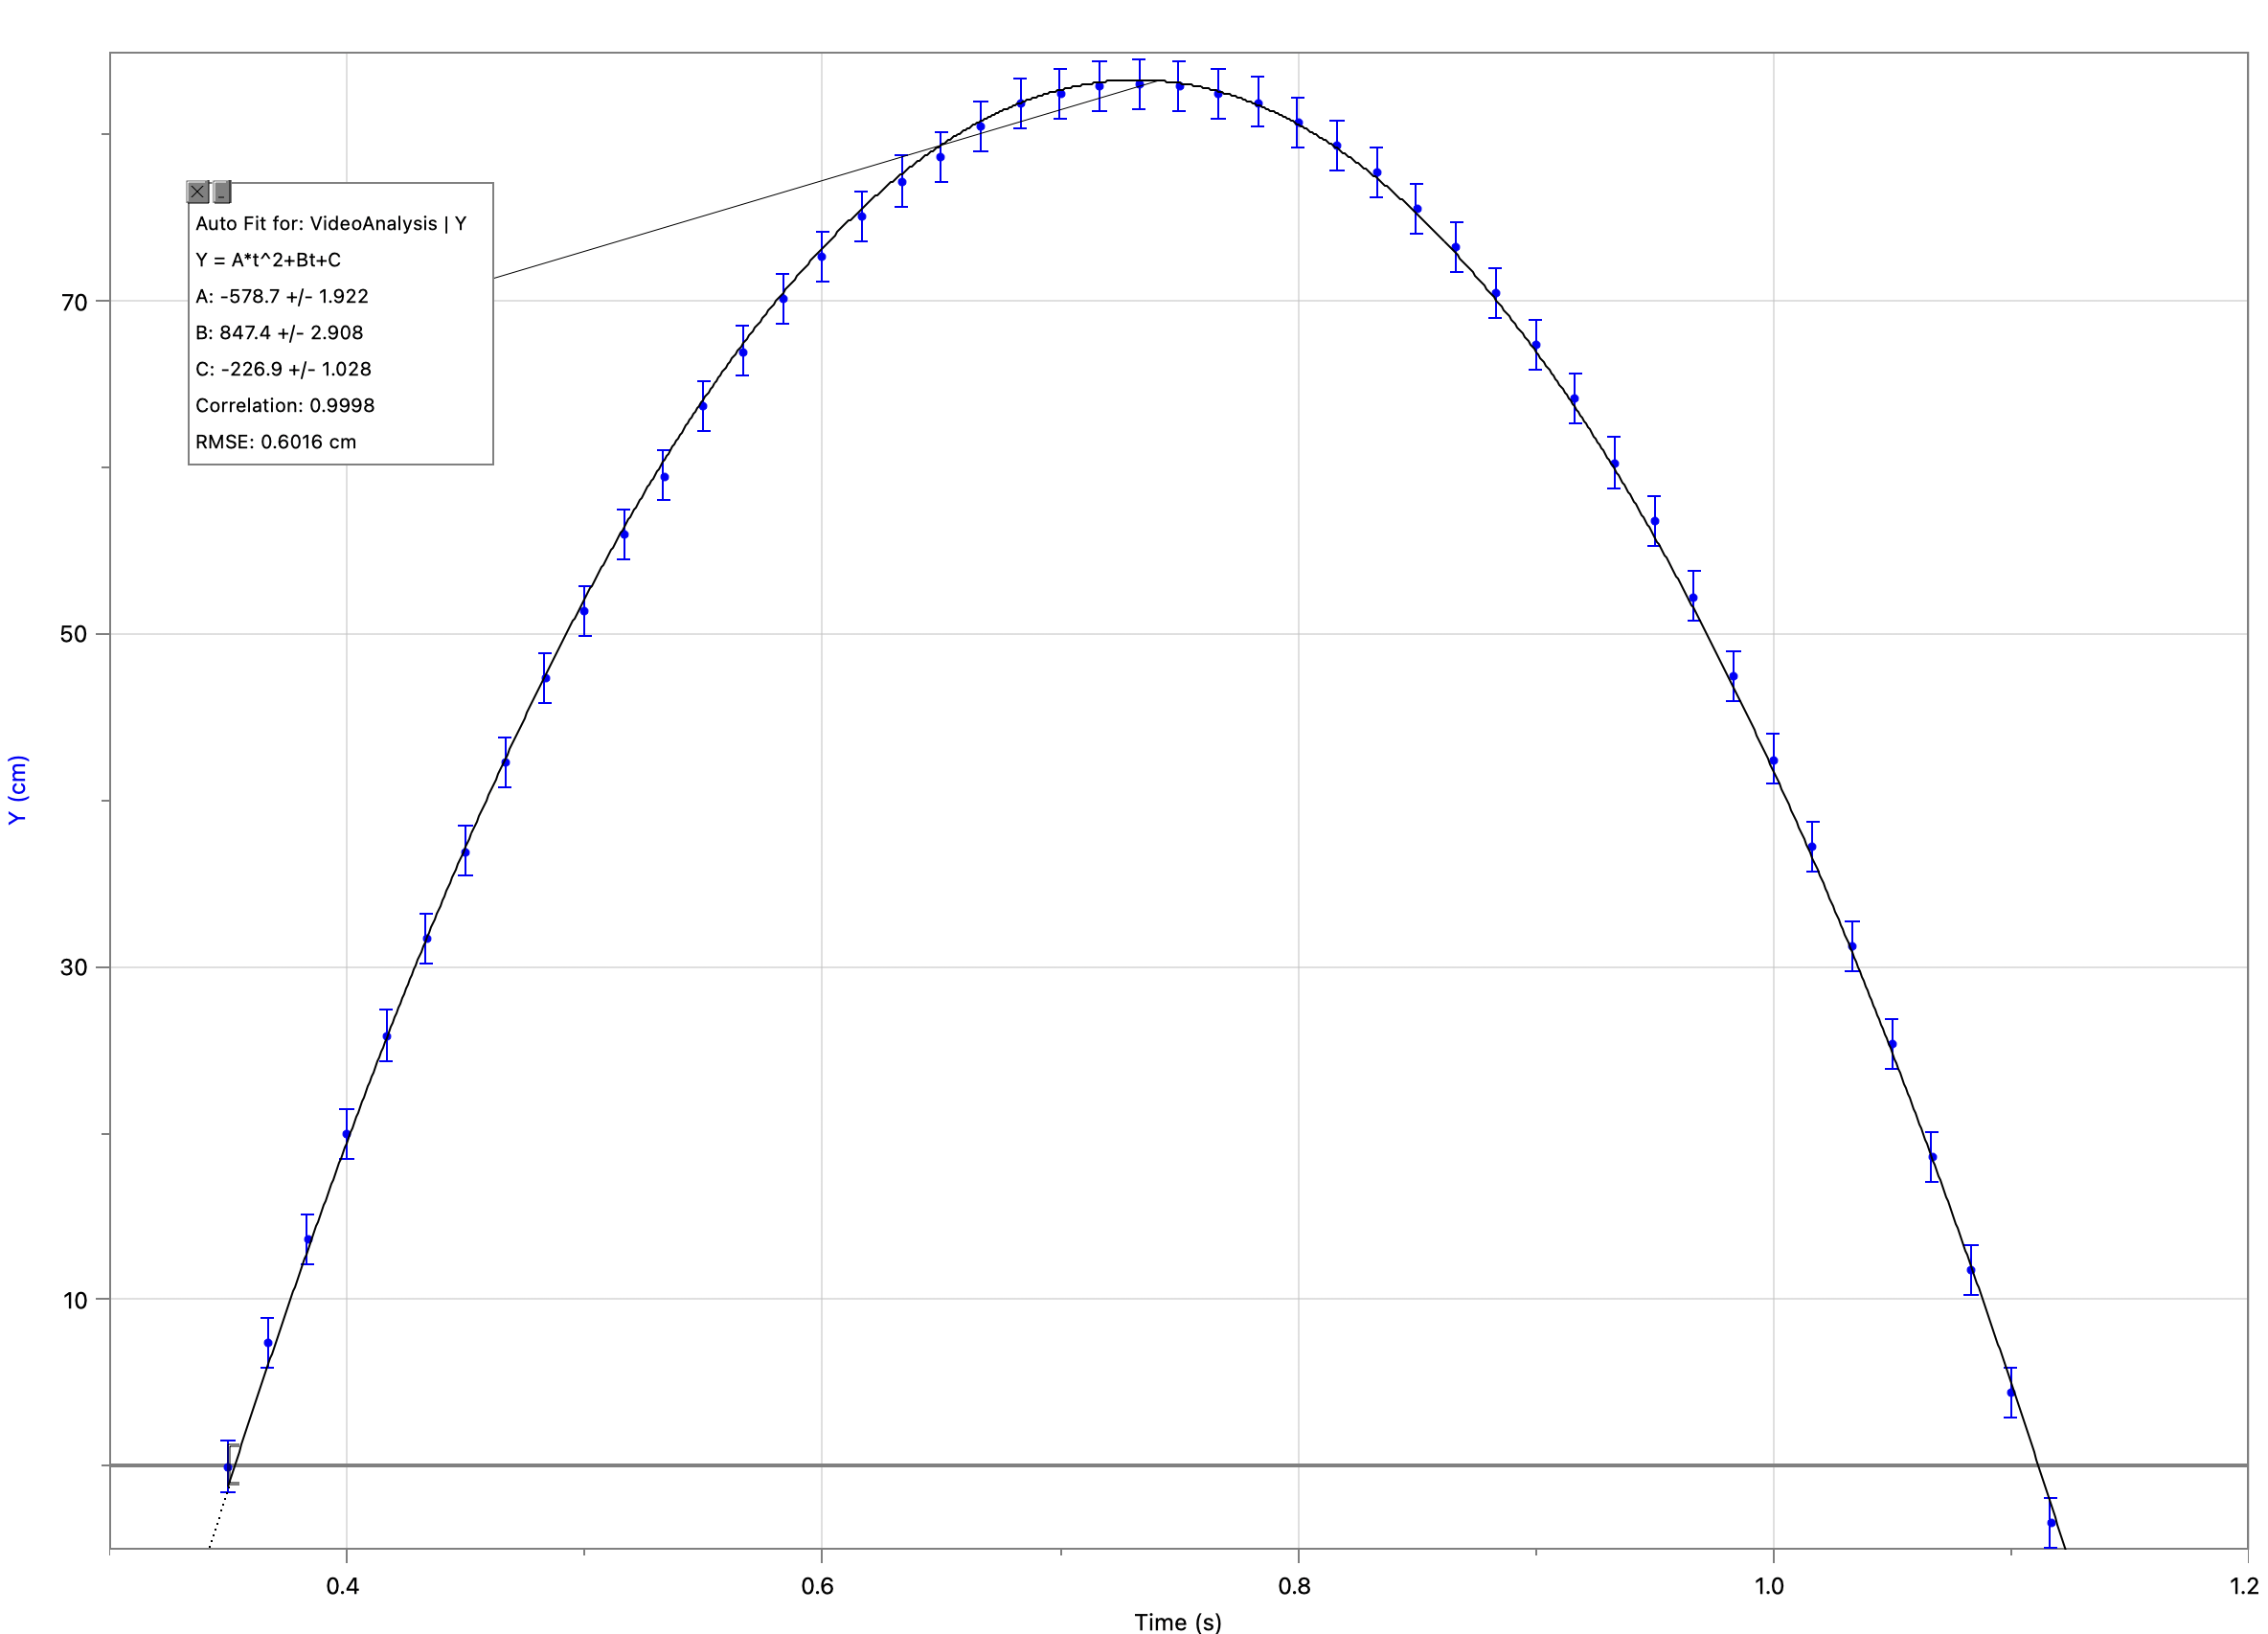
\includegraphics[width=15.9cm, height=10.8cm]{Sy-t.png}
    \caption{\({S_y}\)-$t$ Graph}
    \label{fig2}
\end{figure}
Similar to above, we could determine the relationship between \(S_y\) and \(t\) is
\[
    S_y = -(578.7 \pm 1.922) t ^ 2 + (847.4 \pm 2.908)t -(226.9 \pm 1.028)
\]
\subsubsection{Acceleration}
Logger Pro didn't tell us what the acceleration directly since all that it gave is graphs and data sets. So we would have to deduce it ourselves.\par
To determine the acceleration of $y$, it will first be necessary to obtain the $V_t$-t graph of the motion. Once this has been obtained, the slope of the graph can be used to calculate the acceleration of $y$.
For exact values, we can use the graph shown below. From which we can learn the relationship between $V_y$ and $t$ is
\[
    V_y = -1158 t + 843.4
\]
This means the value of $a$ is equal to $-1158\ cms^{-2}$, and the initial velocity, denoted as $V_i$, is equal to $843.4\ cms^{-1}$.
\begin{figure}[H]
    \centering
    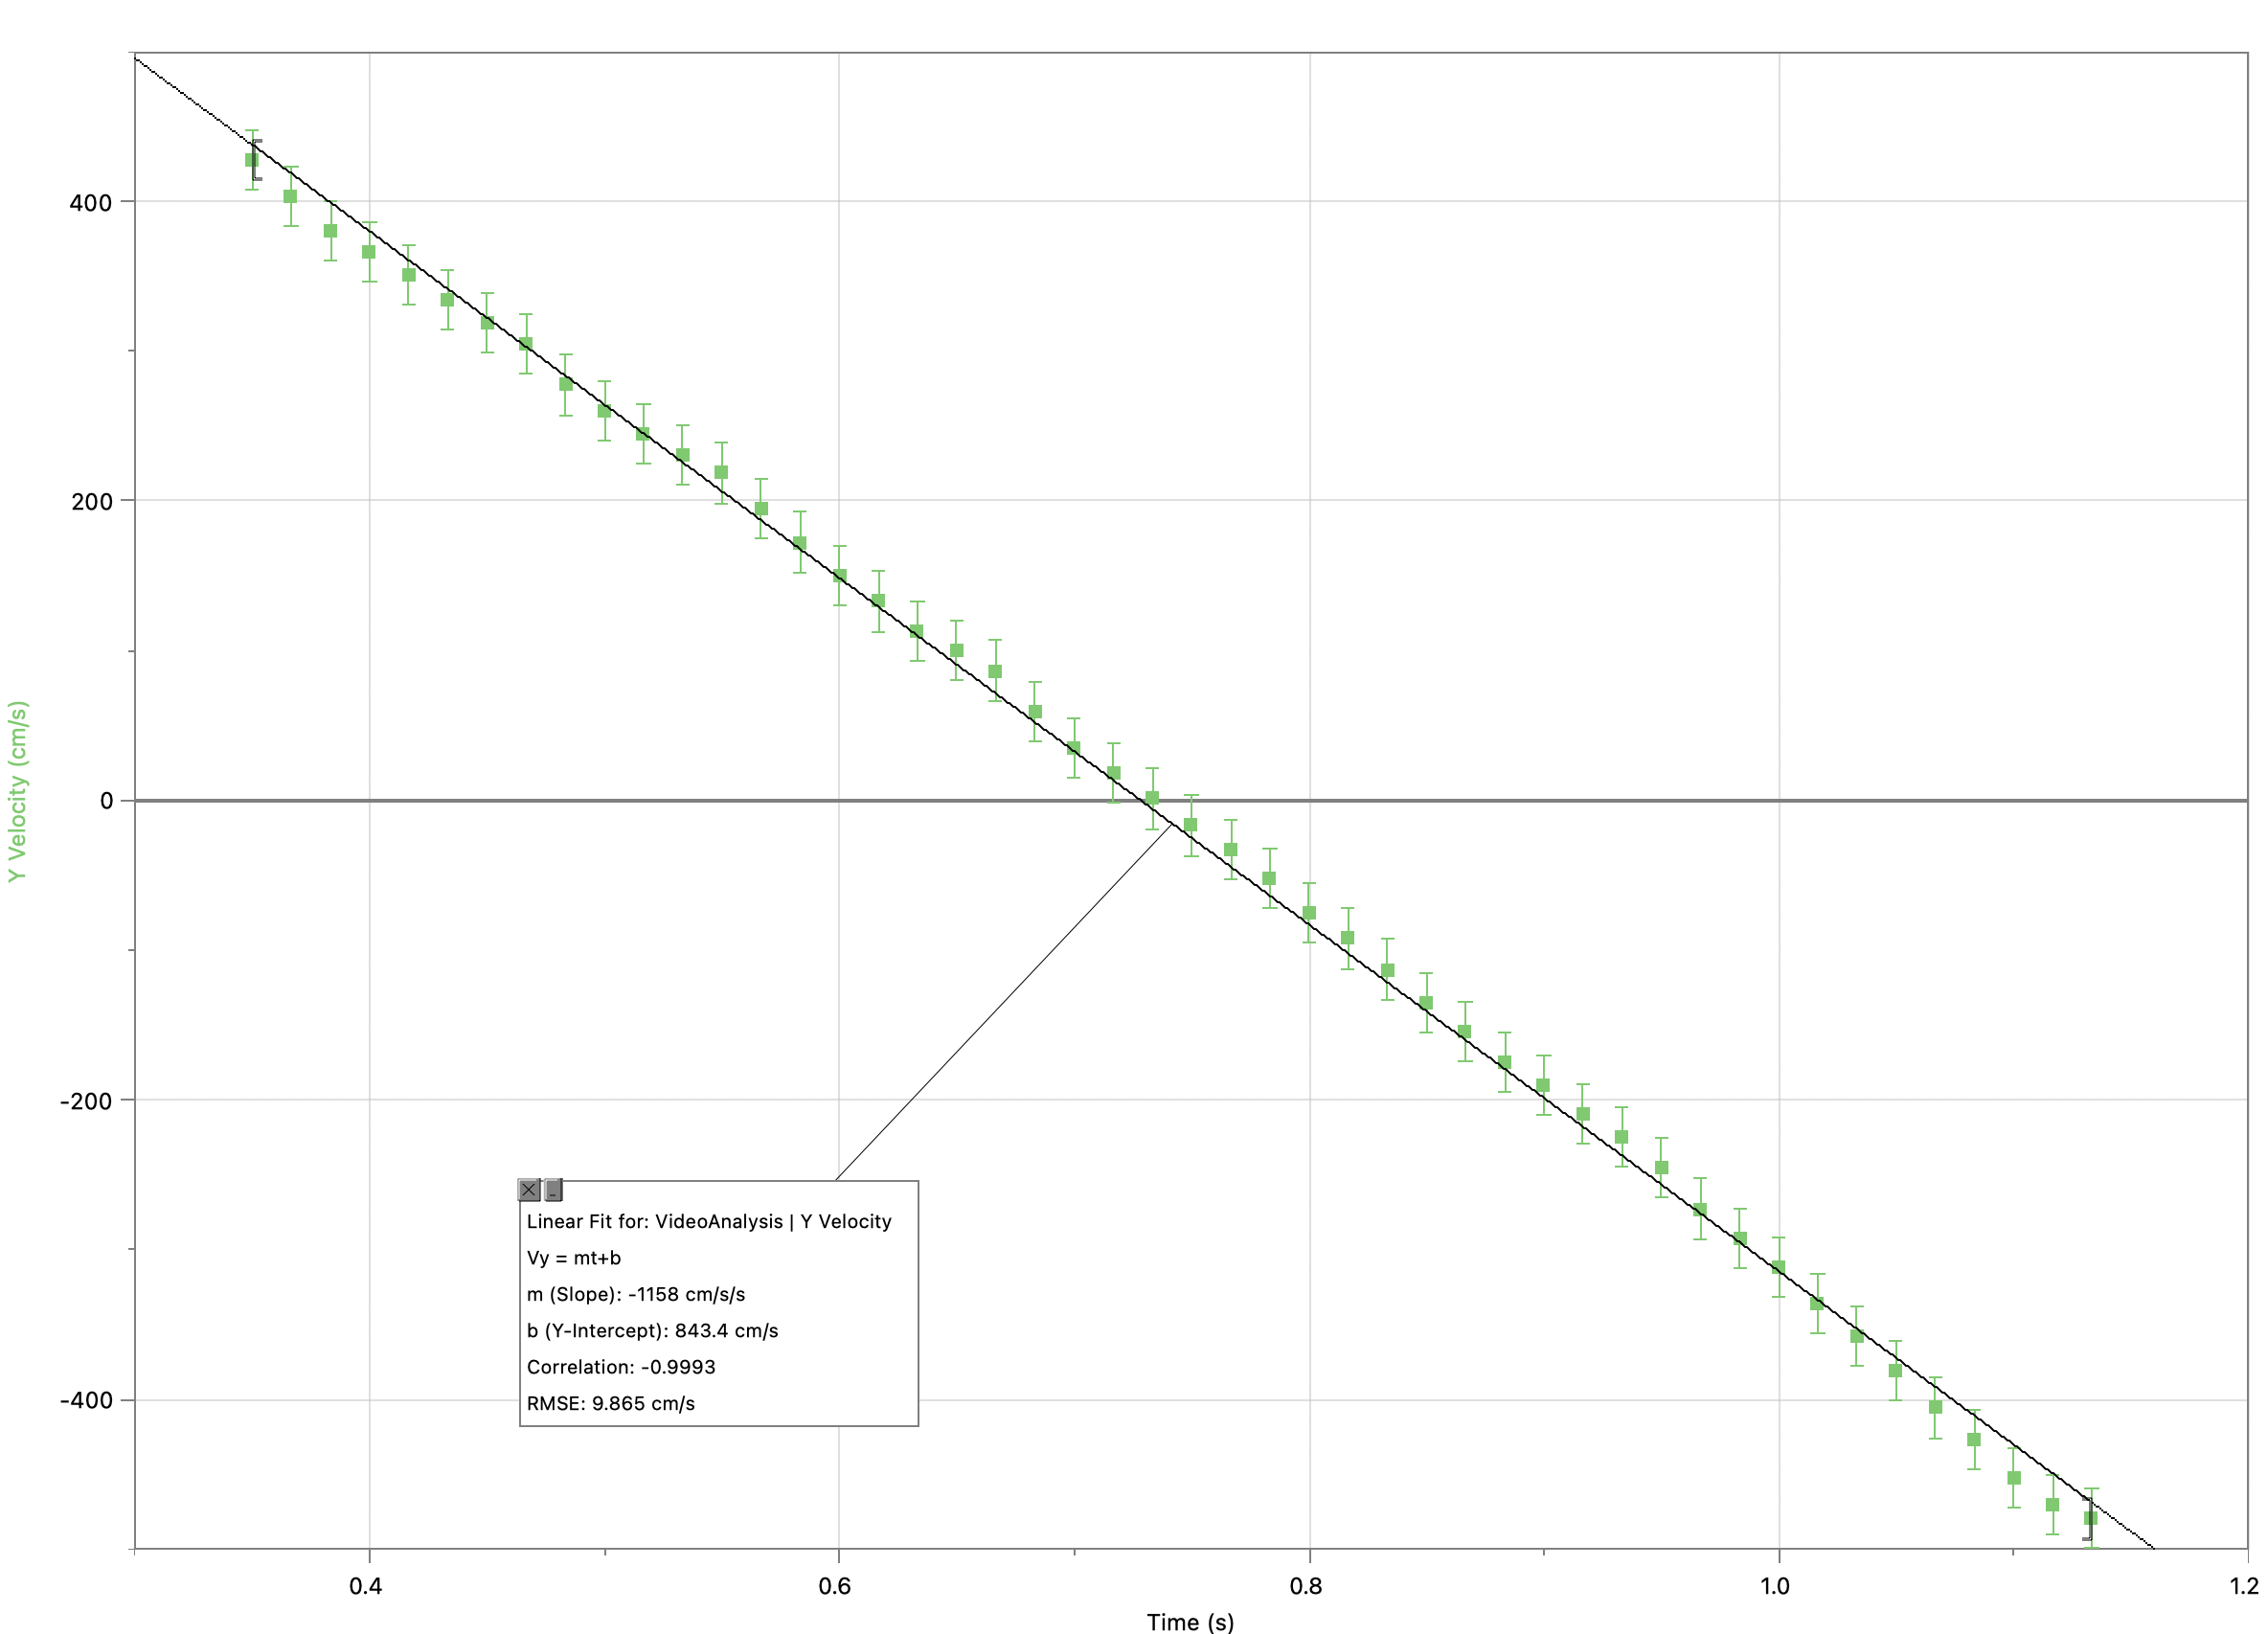
\includegraphics[width=15.9cm, height=10.8cm]{Vy-t.png}
    \caption{\(\rm{V_y}\)-$t$ Graph}
    \label{fig3}
\end{figure}
\section{Conclusion and Evaluation}
\subsection{Conclusion}
Based on the calculations that have been performed and presented above, I have come to the conclusion that the acceleration of y, denoted as \(A_y\) is equal to \(1158\ cm^{-2}\). 
\subsection{Evaluation}
After conducting extensive research on the internet, I have discovered that the gravitational acceleration on Earth is approximately equal to $981\ cms^{-2}$. Furthermore, due to the constant nature of this acceleration, the speed of an object in freefall is directly proportional to the time it spends falling. This discrepancy could be due to a variety of factors, such as environmental conditions, measurement errors, or other unknown variables.
\end{spacing}
\newpage
\section{Appendixes}
\subsection{Data Table}


\begin{longtable}[h]{| c | c | c | c | c |}
    \hline
    t(\(s\))    & x(\(cm\)) & y(\(cm\))  & \(\rm{V}_{x}\)(\(cms^{-2}\)) &\(\rm{V}_{y}\)(\(cms^{-2}\))  \\
    \hline
    \endfirsthead
    \endhead
0.35  & -0.01   & -0.019  & -127.62 & 427.89  \\
0.367 & -2.09   & 7.459   & -129.99 & 403.41  \\
0.383 & -4.42   & 13.667  & -128.85 & 380.77  \\
0.4   & -6.37   & 19.968  & -128.39 & 366.32  \\
0.417 & -8.59   & 25.88   & -132.93 & 351.18  \\
0.433 & -10.85  & 31.74   & -134.34 & 334     \\
0.45  & -13.17  & 36.945  & -129.61 & 318.69  \\
0.467 & -15.21  & 42.329  & -122.36 & 304.83  \\
0.483 & -17.23  & 47.369  & -116.99 & 277.35  \\
0.5   & -18.94  & 51.367  & -121.45 & 260.55  \\
0.517 & -21.16  & 56.035  & -132.72 & 244.97  \\
0.533 & -23.51  & 59.51   & -136.55 & 231.13  \\
0.55  & -25.79  & 63.697  & -135.65 & 218.52  \\
0.567 & -28.03  & 66.992  & -133.33 & 194.74  \\
0.583 & -30.21  & 70.16   & -132.49 & 172.32  \\
0.6   & -32.45  & 72.722  & -131.99 & 149.67  \\
0.617 & -34.56  & 75.058  & -133.77 & 132.84  \\
0.633 & -36.94  & 77.222  & -133.41 & 113.41  \\
0.65  & -39.04  & 78.708  & -131.08 & 100.16  \\
0.667 & -41.31  & 80.545  & -128.19 & 86.66   \\
0.683 & -43.28  & 81.87   & -127.39 & 59.34   \\
0.7   & -45.55  & 82.457  & -127.36 & 35.04   \\
0.717 & -47.5   & 82.89   & -129.4  & 17.92   \\
0.733 & -49.92  & 83.077  & -129.28 & 1.1     \\
0.75  & -51.71  & 82.954  & -133.46 & -16.78  \\
0.767 & -54.3   & 82.457  & -141.16 & -32.42  \\
0.783 & -56.66  & 81.955  & -136.13 & -52.12  \\
0.8   & -58.7   & 80.779  & -137.57 & -75     \\
0.816 & -61.26  & 79.333  & -137.91 & -92.19  \\
0.833 & -63.31  & 77.778  & -138.33 & -112.89 \\
0.85  & -65.79  & 75.599  & -142.76 & -134.87 \\
0.866 & -68.15  & 73.238  & -142.21 & -154.48 \\
0.883 & -70.57  & 70.464  & -139.43 & -174.64 \\
0.9   & -72.82  & 67.348  & -135.16 & -190.5  \\
0.916 & -74.95  & 64.173  & -137.48 & -209.24 \\
0.933 & -77.48  & 60.301  & -136.92 & -224.92 \\
0.95  & -79.54  & 56.758  & -135.79 & -245.37 \\
0.966 & -81.82  & 52.265  & -143.53 & -272.75 \\
0.983 & -84.41  & 47.513  & -146.53 & -292.88 \\
1     & -86.77  & 42.469  & -145.7  & -311.28 \\
1.016 & -89.26  & 37.264  & -144.28 & -335.49 \\
1.033 & -91.68  & 31.243  & -137.88 & -357.99 \\
1.05  & -93.77  & 25.342  & -136.26 & -381.1  \\
1.066 & -96.1   & 18.569  & -141.42 & -405.62 \\
1.083 & -98.49  & 11.757  & -146.88 & -426.8  \\
1.1   & -101.01 & 4.465   & -151.36 & -451.99 \\
1.116 & -103.6  & -3.43   & -152.44 & -469.85 \\
1.133 & -106.12 & -11.505 & -152.01 & -479.49
\label{raw data table}
\end{longtable}


\end{document}